\chapter{Quantum-dot cellular automata}
\label{ch:QCA_intro}
\graphicspath{{../gfx/chapter01/}}


\section{An alternative computing paradigm}
\label{sec:an_alternative_computing_paradigm}

\begin{figure}
  \center
  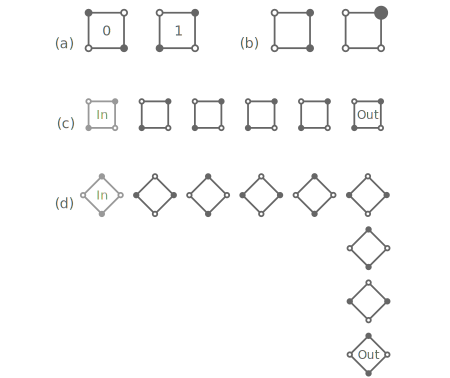
\includegraphics{intro_qca}
  \caption
[Building blocks of quantum-dot cellular automata (QCA) circuitry]
{
\glsreset{QCA}
Building blocks of \cgls{QCA}. (a) A \cgls{QCA} cell consists of four quantum
dots on the corners of a square and is occupied by two electrons. Due to Coulomb
repulsion, two energetically preferred states emerge, logic 0 and logic 1. (b)
Both electrons occupying the edge of the cell or doubly occupying a single
quantum dot are unfavourable high-energy states. (c) A straight line of cells
functions as a wire and transmits a signal. (d) A diagonal line of cells (cells
rotated by $45^{\circ}$) transmits a signal alternating from cell to cell. Wires
can have kinks.
}
  \label{fig:intro_qca}
\end{figure}
%
\begin{figure}
  \center
  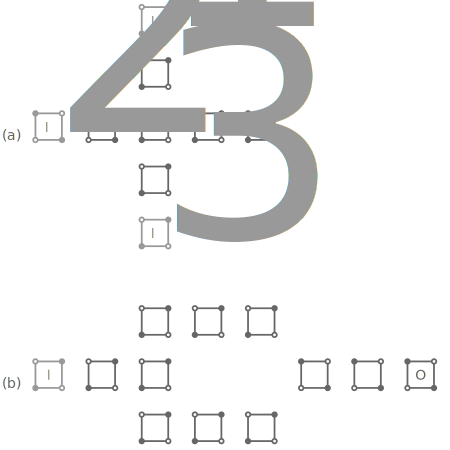
\includegraphics{gates}
  \caption
[QCA gates]
{
\cgls{QCA} gates. (a) The majority gate's three inputs ``vote'' on the output. The gate
is commonly operated with one fixed input, for example $I_3$, and then functions
as an AND ($I_3 = 1$) or OR gate ($I_3 = 0$) for the remaining two inputs. Here
the gate performs the computation $1 \land 0 = 1$. (b) The inverter performs
logical negation, swapping logic 0 for logic 1 and vice versa.
}
  \label{fig:gates}
\end{figure}

\glsreset{QCA}
\glsreset{CMOS}
Lent \emph{et~al}.\ introduced the concept of \cgls{QCA} as an alternative
computing paradigm in 1993 \cite{lent1993quantum}. They devised a novel physical
scheme to build digital circuits that would overcome some of the limitations of
\cgls{CMOS} technology, promising potentially lower power consumption, higher
device density, and faster clocking. As the name suggests, quantum-dot cellular
automata are made from quantum dots that are grouped into cells.
Figure~\ref{fig:intro_qca}(a) shows a basic \cgls{QCA} cell in which four
quantum dots are arranged on the corners of a square. The dots are idealized as
highly localized single orbitals that are perfectly decoupled from some
non-intrusive medium or substrate. Because of the Pauli principle, each dot can
be occupied by zero, one, or two electrons. In the \cgls{QCA} scheme, however,
each cell is occupied by exactly two electrons, and each constituent dot is
quarter-filled on average. The electrons tunnel only weakly between different
dots in a cell, and the dominant energy scale is the Coulomb repulsion between
the particles. Because of the large energy cost to two electrons occupying the
same site or adjacent ones, the diagonal states are the two energetically
preferred electron configurations. In comparison, edge states or doubly occupied
quantum dots are unfavourable higher energy states, see
Fig.~\ref{fig:intro_qca}(b). The two diagonal states can be identified with
logic 0 and 1, respectively. \emph{A priori} the two bit encodings have the same
energy, but this degeneracy can be lifted by an external Coulomb potential,
arising, for example, from a second nearby \cgls{QCA} cell.

A single cell by itself is not very interesting. But multiple cells can be
positioned next to one another, for example as a straight line of cells, as
shown in Fig.~\ref{fig:intro_qca}(c). The approach once again assumes that
Coulomb forces are strong and that electron tunnelling between cells is very
small. For a straight line of cells, the long-ranged, unscreened Coulomb forces
will tend to align the electron configurations of adjacent cells. If the first
cell is in logic state 1, then the second cell will also prefer logic state 1
and so in turn will all the other cells in the line. The situation is the same
for logic state 0. Therefore, a straight line of cells is similar to a wire not
only in geometry, but also in functionality: it transmits a digital signal. The
same is true, with slight modifications, for a diagonal line of cells---cells
rotated by $45^{\circ}$, as illustrated in Fig.~\ref{fig:intro_qca}(d). In this
case, the signal alternates from cell to cell; that is, logic 1 will follow
logic 0 which followed from logic 0, and this again is simply by virtue of the
dominant Coulomb interaction between electrons on different cells. By using an
even number of cells the diagonal line of cells works as a wire just as well as
a straight line of cells. The pictogram also demonstrates a $90^{\circ}$ kink
for the diagonal line of cells, which our newly gained intuition for these
Coulomb-driven systems expects to pose no problem for signal transmission.

The main idea of the \cgls{QCA} approach becomes apparent: ideal, bistable cells
interact with each other solely by Coulomb repulsion. By arranging the cells in
clever geometries, we can realize interesting functionalities. The idea as such
is quite general and does not strictly rely on the two-electron--four-dot cell
introduced above. Indeed, a number of variations exist, such as cells consisting
of two dots and occupied by only one electron that interact via dipole fields
instead of quadrupole fields as for the conventional cells. Another variation is
a four-dot cell with six electrons---two holes---instead of two electrons. Even
the interaction need not be Coulombic. For example, magnetic \cgls{QCA} schemes
have been explored \cite{bernstein2005magnetic}. While \cgls{QCA} carries
``quantum'' in its name and is sought to be implemented at the nanoscale, the
approach operates close to the classical limit. The Coulomb interaction
dominates with the tunnelling of electrons serving as a small perturbation,
which nonetheless drives the system's dynamics. The approach is insensitive to
the spin degrees of freedom. Let us finally note that \cgls{QCA} is a not a
cellular automata in a strict mathematical sense, but only by analogy to the
idea of cells evolving according to simple rules that depend on neighbouring
cells.

One clever geometrical cell arrangement, the majority gate, is shown in
Fig.~\ref{fig:gates}(a). The gate has three inputs which ``vote'' on the central
cell. The majority wins and sets the single output. The device is commonly
operated with one fixed input, for example $I_3 \doteq 0$ or $I_3 \doteq 1$. In
the first case, with $I_3 \doteq 0$, the device functions as an AND gate for the
remaining two inputs, $O = I_1 \land I_2$. In the second case, with $I_3 \doteq
1$, it is an OR gate with $O = I_1 \lor I_2$. The figure shows the gate
performing the computation $1 \land 0 = 1$. Now the only missing piece for
Boolean algebra is negation, $O = \lnot I$. We had already seen that simply
arranging cells at an $45^{\circ}$ angle as in the diagonal line of cells
negates the signal from cell to cell. The inverter, shown in
Fig.~\ref{fig:gates}(b), recasts this idea into a more robust layout. With that
we have, at least in principle, all the necessary building blocks for Boolean
algebra and thus digital circuitry.

Conceptually, it is most elegant to set the inputs for a \cgls{QCA} circuit via
driver cells---cells that resemble the \cgls{QCA} cell in form, but are made up
of static point charges instead of quantum dots. These static charges are
thought to be manipulable to vary the input smoothly from the logic 0 to the
logic 1 state. In Figs.~\ref{fig:intro_qca}~and~\ref{fig:gates}, these driver
cells are represented in light grey. Of course, in practice such driver cells
would be difficult if not impossible to implement and the inputs are more likely
set by leads that provide the necessary perturbative electrostatic fields. The
output of a \cgls{QCA} device can be directly read from its output cells. In
practical implementations this will require a non-trivial charge probing
apparatus. Changing the input for a \cgls{QCA} device throws the system into an
excited, non-equilibrium state. The system will then dissipatively propagate to
its new ground state. For the given inputs, this ground state corresponds to the
solution of the computational problem the circuit is designed to solve. Let us
emphasize this: in \cgls{QCA}, the computational solution maps directly to the
physical ground state. While the computation is being performed, only a few
charges move locally, in each cell. Operating close to the ground state,
\cgls{QCA} is thus a truly current-free approach and consequently inherently
low-power, especially when compared with \cgls{CMOS} technology. But the
operation close to the ground state also raises concerns for the operational
temperature for these devices. It is clear that for real-world applications we
would want to engineer the system so that the energy gap between the ground
state and the low-lying excited states far exceeds room temperature. Different
material systems provide different dissipative channels, and modelling them
quantitatively or even qualitatively correctly is very challenging. As a
consequence, it is difficult to derive general expectations for the clocking
speed of \cgls{QCA} circuits. The switching speed of a majority gate, for
example, will greatly depend on the system's parameters, but particularly on the
nature of the dissipative coupling of the circuit to its environment. A small
dissipative coupling will have the output polarization oscillating before it
eventually settles to its correct value. A very dissipative system in contrast
might get stuck in meta-stable states. 

\cgls{QCA} circuits consist of wires, gates, and other structures arranged on a
two-dimensional surface---very similar to conventional electronics devices.
However, the structures themselves are quasi-one-dimensional, and this poses a
challenge for building large-scale \cgls{QCA} circuits. A good example is a
single long wire, which is truly one-dimensional. When we think about switching
the input for the wire, we think of the information being propagated as a charge
density wave along the line of cells, or, equivalently, as propagating the
domain boundary between logic 0 and logic 1. This domain boundary incurs an
energy cost that the system seeks to minimize, causing the wire to order. For an
increasingly longer wire, however, the gain in entropy for moving a domain
boundary freely throughout the wire ($S \sim \log N$, $N$ the number of cells)
soon exceeds the loss in energy, which is reflected by the free energy of the
system ($F = U - T S$). Quite generally, a one-dimensional system with discrete
(rather than continuous) degrees of freedom cannot be ordered in the
thermodynamic limit except at zero temperature. Therefore, the
finite-temperature, infinitely long wire will always exhibit exponentially
decaying bit correlations and thus be unable to transmit a signal. The gap
between the first excited state---with two domains---and the completely ordered
ground state, together with the desired operational temperature will determine
the maximum system size.

\begin{figure}
  \center
  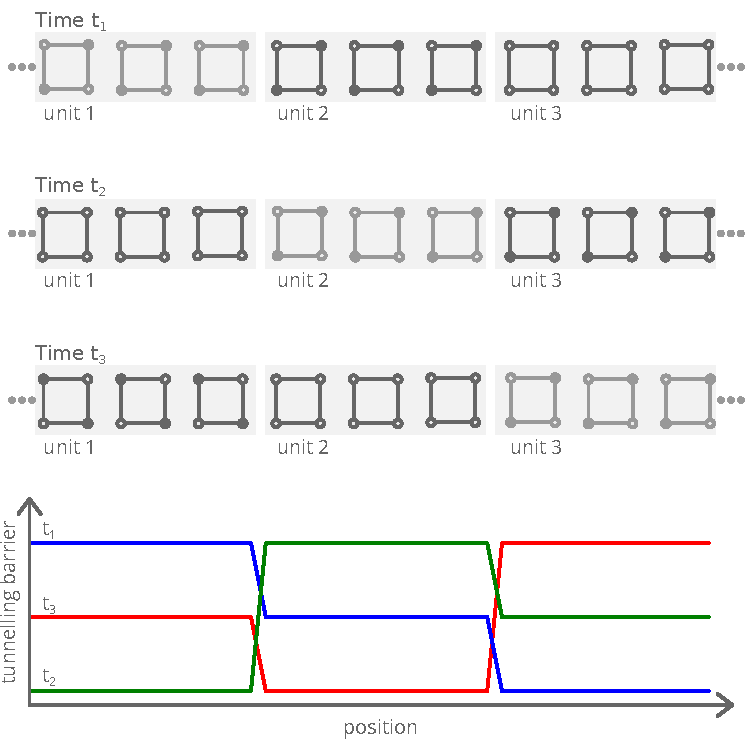
\includegraphics{clocking}
  \caption
[Clocked QCA for a line of cells]
{
Clocked \cgls{QCA} for a line of cells. To avoid entropy-induced disorder in large \cgls{QCA}
circuits, the system is partitioned into smaller units, labelled 1, 2, and 3 in
this example. By varying the tunnelling barriers, each unit is put through the
three phases \emph{frozen} (high barrier, light grey cells), \emph{active}
(medium barrier, dark grey cells), and \emph{delocalized} (low barrier, dark
grey cells with empty dots). Synchronizing the phases of adjacent units allows
to pipeline information flow and computations. The line of cell's three units
and their tunnelling barriers are shown at three different times, $t_1<t_2<t_3$.
A logic 1 state is propagated from the left to the right. At $t_3$ a logic 0
state is coming in from the left.
}
  \label{fig:clocking}
\end{figure}

To address this scaling problem, we partition large circuits into smaller units.
The size of each unit is chosen to be small enough to avoid entropy-induced
disorder at a given operational temperature. Each unit can be turned ``on'' and
``off'' separately: ideally, individual gates would allow one to effectively
raise and lower the tunnelling barriers between quantum dots in each unit and
thus provide a mechanism to freeze or delocalize the electrons. A unit with
\emph{frozen} electrons can serve as the input for a unit with more
\emph{active} charge carriers, which works like a regular \cgls{QCA} circuit. A
unit with completely \emph{delocalized} electrons, in contrast, will not
influence adjacent units. By putting each unit through the three phases
\emph{delocalized}, \emph{active}, and \emph{frozen} and synchronizing adjacent
units appropriately, we can control the information flow through the system very
nicely, as illustrated in Fig.~\ref{fig:clocking}. Therefore, by partitioning
the circuit and introducing a clocking scheme, we not only handle the scaling
problem but also arrive at a pipelining architecture. If and how the tunnelling
barriers can be effectively modified will depend on the details of the specific
\cgls{QCA} implementation. Also, in practice the \cgls{QCA} circuit units cannot
be too small as they must be individually addressable. Gates which turn
\cgls{QCA} units ``on'' and ``off'' provide another potential benefit as well.
We are able to control how and especially how fast the gate voltage is changed
and should be able to tune it with respect to the inherent time scales of the
\cgls{QCA} system, which are set by the system's parameters and the dissipative
coupling to its environment. This should afford a better control over the
dynamics of the switching process and might help mitigate problems such as
oscillating outputs and meta-stable states, mentioned above
\cite{lent1997device}.


\section{Atomic silicon quantum dots}
\label{sec:atomic_silicon_quantum_dots}

\newacronym{DB}{DB}{dangling bond}
\newacronym{STM}{STM}{scanning tunnelling microscope}

\begin{figure}
  \center
  \includegraphics{silicon}
  \caption
[Atomic silicon quantum dots]
{
\glsreset{STM}
\glsreset{DB}
Atomic silicon quantum dots are \emph{\cglspl{DB}} on a hydrogenated
(100) silicon surface. (a) A \cgls{STM} image of an
atomic silicon quantum dot \cgls{QCA} cell. (b) Band diagram of a \cgls{DB} on a strongly
n-doped silicon substrate. (c) The reconstructed (100) hydrogenated silicon
surface, showing dimer rows. (d) Two closely spaced tunnel-coupled \cglspl{DB} perturbed
by a third \cgls{DB}. The top right \cgls{DB} is seen to be more negatively charged than the
other \cgls{DB} of the closely spaced pair, due to Coulomb repulsion from the
perturbing third \cgls{DB} in the bottom left. All \cgls{STM} images and \emph{ab initio}
estimates from Wolkow \emph{et~al}.\ \cite{wolkow2013silicon} \cite{pitters2011tunnel}.
}
  \label{fig:silicon}
\end{figure}

\glsreset{STM}
\glsreset{DB}
Our objective is the general, rather than implementation-specific,
characterization of the \cgls{QCA} approach. Even so, it is still important to
consider concrete experimental realizations, not only as a motivation for our
work, but also to put our modelling and results into context. One of the most
promising and recent experimental implementations of \cgls{QCA} is based on
atomic silicon quantum dots, and we will therefore use them as our experimental
reference. Atomic silicon quantum dots were first demonstrated as a possible
\cgls{QCA} implementation by Wolkow \emph{et~al}.\ in 2009, when the group first
constructed a single \cgls{QCA} cell. Figure~\ref{fig:silicon}(a) shows a
\cgls{STM} image of their device. Since then impressive advances have been made
both in the understanding of the electronic properties of these quantum dots as
well as in the precise fabrication of larger \cgls{QCA} structures. With
atomic-scale feature sizes, this experimental system promises room temperature
operation, while at the same time tapping into the established and highly
sophisticated silicon technology. Being based on silicon should also ease
integration with existing \cgls{CMOS} circuitry.

Atomic silicon quantum dots are \emph{dangling bonds} on a hydrogen-terminated
$(100)$ silicon surface. Atoms on a $(100)$ silicon surface have two unsatisfied
bonds. Pairs of surface atoms form dimers, satisfying one bond. The remaining
bond is satisfied by passivating the surface with hydrogen.
Figure~\ref{fig:silicon}(c) shows a \cgls{STM} image of the reconstructed
silicon surface, where the dimer rows are clearly visible and the dimensions are
indicated. By applying a relatively large current through the \cgls{STM} tip,
individual hydrogen atoms can be removed, with atomic precision. This leaves a
\emph{\cgls{DB}} that acts as a quantum dot: energetically, electrons on the
\cgls{DB} orbital sit in the silicon band gap and are therefore decoupled from
the silicon substrate. Figure~\ref{fig:silicon}(b) shows the band diagram of a
\cgls{DB} on an n-doped substrate. Chemically, \cglspl{DB} have proven to be
surprisingly robust with respect to environmental molecules. From \emph{ab
initio} calculations it is known that the sp$^3$ \cgls{DB} orbital extends
predominantly into the bulk and only a little into the vacuum. The orbital's
lateral extent is on the order of 1~nm and therefore spans multiple silicon
lattice atoms. Due to orbital overlap, closely spaced \cglspl{DB} are
tunnel-coupled. A neutral \cgls{DB} consists of the positive silicon ion and one
electron. In the experimentally common strongly n-doped system, the \cgls{DB}
accepts one more electron and is therefore $-1e$ negatively charged. Conversely,
in a p-doped sytem the \cgls{DB} will donate its electron and become $+1e$
positively charged. The Coulomb repulsion between negatively charged \cglspl{DB}
can be used to adjust the filling of \cgls{DB} assemblies simply by controlling
the \cglspl{DB}' positions. For example, on an n-doped substrate two \cglspl{DB}
may eject one electron (which goes back to the bulk) and share the remaining
single electron, when placed close enough together. To prove this, a third
\cgls{DB} is placed close by, but not close enough to be tunnel-coupled. The
effect of the Coulomb repulsion can be seen via \cgls{STM} imaging,
Fig.~\ref{fig:silicon}(d), where the \cgls{DB} farthest from the perturbing
external charge is more negatively charged (darker in the \cgls{STM} image) than
the closer \cgls{DB}. The observed charge shift is only possible when both
closely-spaced \cglspl{DB} share a single electron. To form the previously shown
\cgls{QCA} cell, Fig.~\ref{fig:silicon}(a), on a strongly n-doped silicon
substrate four \cglspl{DB} are brought close enough together so that two
electrons go back to the bulk, leaving the cell with six electrons (two holes)
in total and a cell net charge of $-2e$, which is the right charge regime for
\cgls{QCA}.

Atomic silicon quantum dots provide some examples of how a real world system
might be different from the idealized picture we typically employ to describe
the \cgls{QCA} approach. We like to think of quantum dots as highly localized
orbitals. But in the silicon system the orbitals of the \cglspl{DB} actually
span multiple lattice sites and only if the \cglspl{DB} are placed far enough
apart might we still be able to consider them as localized. We do not consider
the substrate but treat quantum dots as perfectly isolated entities. Of course,
in practice the substrate will certainly influence the \cgls{QCA} device. In the
silicon system, free charge carriers will screen the long-ranged Coulomb
interactions that the \cgls{QCA} scheme relies on, although likely on scales
larger than the circuit feature size. The screening is not necessarily
disruptive for \cgls{QCA} and might even be beneficial, for example by
minimizing charge buildup in large systems. But to quantify the screening
accurately it is necessary to thoroughly understand and precisely model the
system; for atomic silicon quantum dots, which live at the surface, that would
surely be very challenging. The silicon substrate could also, conceivable,
provide a second tunnelling channel between \cglspl{DB}. In addition to
electrons hopping directly from \cgls{DB} to \cgls{DB} they could first tunnel
from \cgls{DB} to substrate and then back to another \cgls{DB}. Therefore an
accurate model for atomic silicon quantum dots might need to accommodate the
nature of the \cgls{DB} orbitals, screening, multiple tunnelling channels, and
possibly other effects.


\section{The extended Hubbard model}

\cgls{QCA} systems are typically modelled by an extended Hubbard Hamiltonian.
The Hubbard model originated in the early 1960s to describe rare-earth systems
with highly localized d- and f-electrons and has since then, of course, become
one of the most widely studied and successful models in condensed matter physics
\cite{Hubbard1964}. In basing our description on the Hubbard model we already
put some key assumptions in place. For example, we assume that the quantum dots
are similar to the highly localized d-orbitals. As discussed above, depending on
the particular \cgls{QCA} implementation this might or might not be a good
description. However, our interest is not in the precise details of any
particular material system; rather, our aim is to investigate universal
characteristics of \cgls{QCA} systems. As long as a \cgls{QCA} system can be
broadly qualitatively described by Hubbard physics---and most prospective
\cgls{QCA} implementations fall into this category---our modelling and findings
should be valid. Conversely, for implementations that are decidedly not
Hubbard-like, our results might not be applicable. An idealized but
semi-realistic description is what we want and for that the Hubbard model is
indeed an appropriate---and tractable---starting point. Specifically, the
Hamiltonian we use is
\begin{equation}
\begin{split}
  \label{eq:H_QCA}
  H =
    &- \sum_{ij\sigma} t_{ij} \, c^{\dagger}_{i\sigma} c_{j\sigma}
    + U \sum_i n_{i\uparrow} n_{i\downarrow}
    - \mu \sum_{i\sigma} n_{i\sigma} \\
    &+ \sum_{i<j} V_{ij} \left( n_{i\uparrow} + n_{i\downarrow} - q \right) 
                        \left( n_{j\uparrow} + n_{j\downarrow} - q \right) \, ,
\end{split}
\end{equation}
where $c^{\dagger}_{i\sigma}$ ($c_{i\sigma}$) creates (annihilates) an electron
on quantum dot $i$ with spin $\sigma$ and the particle number operator is
$n_{i\sigma} = c^{\dagger}_{i\sigma} c_{i\sigma}$. The overlap integral between
dots $i$ and $j$ is denoted by $t_{ij}$, $U$ is the Hubbard on-site Coulomb
repulsion, $\mu$ the chemical potential, and $V_{ij}$ the long-ranged Coulomb
interaction, which is characteristic for \cgls{QCA} systems. For simplicity the
Coulomb term is chosen to be $V_{ij} = \frac{1}{r_{ij}}$ where $r_{ij}$ is the
distance between the two dots $i$ and $j$. We also introduce the
\emph{compensation charge} $q$ which is thought to represent a possible positive
ion at each quantum dot site. This constant positive charge allows us to tune
the net cell charge. For two electrons per cell, for example, $q=0$ yields a net
cell charge of $-2e$ whereas $q = \frac{1}{2}$ represents zero net cell charge.
The $q = \frac{1}{2}$ charge neutral cells are perfect electrostatic
quadrupoles.

The geometric layout of the \cgls{QCA} system and therefore its functionality is
encoded in the hopping parameter $t_{ij}$ and the long-ranged Coulomb term
$V_{ij}$. For the hopping parameter, we usually only consider nearest-neighbour
hopping $t$ and specifically no hopping between the cells. While this constraint
is not strictly necessary for \cgls{QCA}, it is in line with the approach's
underlying idea and greatly simplifies calculations. Because the overlap
integral decays exponentially with distance, as long as the distance between
dots from different cells is larger than the distance between dots within one
cell, the assumption will introduce only a small error. Still, this is something
to keep in mind if we place cells very close to each other. Note that without
inter-cell hopping we can decompose the Hamiltonian into purely Coulombic
cell-cell interaction terms $H^{cc}_{kl}$ and single cell terms $H^c_k$, which
capture the kinetics as well as the inside-cell Coulomb interactions,
\begin{equation}
  \label{eq:H_cell}
  H = \sum_k H^c_k + \sum_{k<l} H^{cc}_{kl} \, ,
\end{equation}
where $k$ and $l$ number the cells. 

\begin{figure}
  \center
  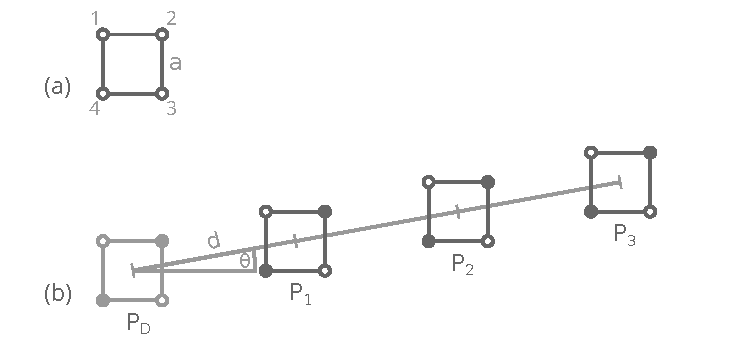
\includegraphics{short_wire}
  \caption
  [Parameterizing QCA layouts]
  {Parameterizing \cgls{QCA} layouts. (a) The edge length of a \cgls{QCA} cell is
  denoted by $a$. The dots of each cell are numbered clockwise. (b) A
  three-cell wire. The cell-cell distance is denoted by $d$, the cell-cell angle
  by $\theta$. The wire's input is set by the driver cell's polarization $P_D$,
  the active cells' polarizations are $P_1$, $P_2$, and $P_3$.}
  \label{fig:short_wire}
\end{figure}

To parameterize the Coulomb term $V_{kl}$ and specifically $r_{ij}$, the
distance between quantum dots $i$ and $j$, we introduce the cell edge length $a$
and the cell-cell distance $d$, as illustrated in
Fig.~\ref{fig:short_wire}(a)~and~(b), where we have used a short line of cells
as an example \cgls{QCA} system. The angle between adjacent cells is denoted by
$\theta$. Ideally each cell should be in logic state 0 or logic state 1, but, of
course, in practice a cell can be in any superposition of the two states or even
in a different state altogether. The \emph{cell polarization} $P_k$ quantifies
the state of the cell, \begin{equation} \label{eq:polarization} P_k =
  \frac{1}{2} \left( n_{4k+2} + n_{4k+4} - n_{4k+1} - n_{4k+3} \right) \, ,
\end{equation} where the dots in each cell are numbered clockwise as indicated
in the figure. We have also introduced the shorthand notation $n_i =
n_{i\uparrow} + n_{i\downarrow}$. The cell polarization is $P_k = -1$ for a
logic 0 and $P_k = +1$ for a logic 1 state. Without any external input the
polarization of a cell will be $P_k = 0$. In the example line of cells, the
input is set via the driver cell's polarization $P_D$ at the left end. The
driver cell's four static point charges are adjusted to reflect the desired
polarization $P_D$. For \cgls{QCA}, the cell polarization really is the
observable of utmost interest. It indicates whether a cell is more in logic
state 0 or logic state 1 and how polarized the cell is, where ideally it should
always be fully polarized, $|P_k| = 1$. In short, the cell polarizations will
indicate how well the \cgls{QCA} approach works for a given system and,
unsurprisingly, calculating cell polarizations for various geometric layouts
over a wide range of system parameters will be our main focus.

The \cgls{QCA} cell is characterized by three energy scales: the
nearest-neighbour hopping $t$, the nearest-neighbour Coulomb repulsion $V_1 =
\frac{1}{a}$, and the on-site Coulomb repulsion $U$. For \cgls{QCA} operation,
$U$ is usually assumed to be large enough that doubly occupied states are gapped
out. We can introduce $V_0 = \frac{1}{\sqrt{2} a}$, the energy scale for
next-nearest-neighbour Coulomb repulsion, which is realized when both electrons
sit diagonally at opposing corners of the cell---our preferred $P_k=\pm1$
states, ideally the ground state. Conversely, $V_1$ corresponds to both
electrons occupying the edge of the cell. Again, for \cgls{QCA} operation we
would like the edge states to be sufficiently gapped out. In other words, the
energy gap, 
\begin{equation}
  \label{eq:deltaV}
  \Delta V = V_1 - V_0 = \frac{2 - \sqrt{2}}{2} \frac{1}{a} \approx 0.3 V_1
\end{equation}
should be large compared to temperature $\Delta V \gg T$, and similarly $U \gg
\Delta V \gg T$. The competition between temperature $T$ and $V_1$ will thus
directly influence how polarized a cell is. In addition, $V_1$, which seeks to
order the cell, will compete with $t$, which delocalizes and disorders the
electrons. \cgls{QCA} is thought to function in a regime where Coulomb is the
dominant energy scale and hopping is a small perturbation: the ratio $V_1/t$ is
large. But it is also clear that if $V_1/t$ becomes too large, for example by
taking $t \rightarrow 0$, the system slows down and eventually freezes, which is
rather undesirable for \cgls{QCA} operation as well. In essence we can describe
a cell by the ratios $V_1/t$, $U/t$, and $T/t$. By similarly expressing the
cell-cell distance in units of the cell size $d/a$, we characterize any
\cgls{QCA} system in dimensionless units.


\section{Basic characterization}
\label{sec:basic_characterization}

\begin{figure}
  \center
  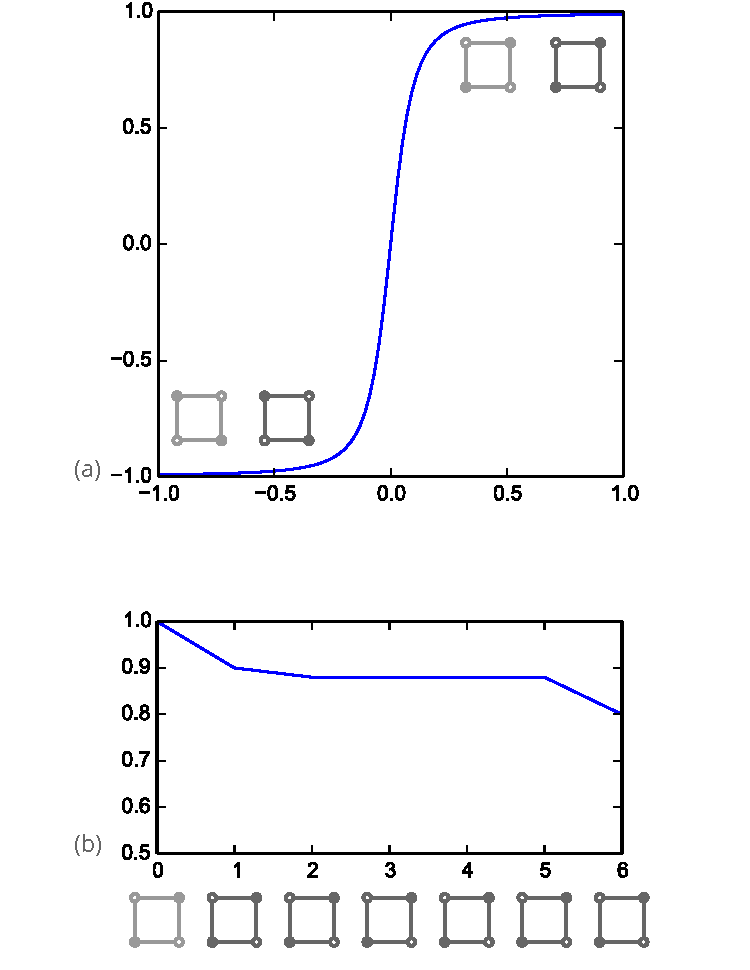
\includegraphics{qca_characterization}
  \caption
[Basic characteristics of QCA devices]
{
Basic characteristics of \cgls{QCA} devices, schematically. (a) The response of a
cell's polarization to a driver cell's polarization is non-linear and exhibits
gain. This gain has been used extensively to argue for the \cgls{QCA} approach's
inherent robustness. (b) Cell polarizations of a six-cell wire with input
polarization $P_D = 1$, as calculated with the intercellular Hatree
approximation. Most cells are polarized with the same saturation polarization
and only the leftmost and rightmost cells deviate slightly. In this picture, the
output polarization does therefore not depend on the wire length.
}
  \label{fig:qca_characterization}
\end{figure}

At the time of this writing, the \cgls{QCA} idea is over twenty years old.
Naturally, the fundamental building blocks of \cgls{QCA} circuitry such as the
single cell itself, the wire, and the majority gate have been characterized.
Interestingly, time-independent properties were investigated relatively briefly
and arguably not exhaustively. The bulk of the existing theoretical work soon
came to focus on system dynamics, the building of large-scale computing
architectures with the \cgls{QCA} paradigm, and specific potential experimental
implementations. Previous work on the characterization of time-independent
\cgls{QCA} properties yielded two main results. First, the cell-cell response,
that is, how the polarization of one cell responds to the polarization of a
neighbouring cell, was established to be non-linear and exhibit gain
\cite{lent1993quantum}. Therefore, even an only partially polarized cell would
fully polarize the cell next to it, Fig.~\ref{fig:qca_characterization}(a). Of
course, gain is highly desirable, if not essential, for building digital
circuits. It compensates for any loss or imperfections and makes the scheme
overall robust. Not coincidentally, \cgls{CMOS} technology is built around the
\cgls{MOSFET} transistor with gain as one of its intrinsic properties. Second,
lines of cells were seen to be polarized with an almost constant polarization
throughout the whole line, Fig.~\ref{fig:qca_characterization}(b)
\cite{lent1993lines}: apart from a few cells next to the driver cell, all
remaining cells in the line would be polarized with the same \emph{saturation
polarization}. As a consequence, the output polarization should not depend on
the number of cells in the line. The saturation polarization was observed to be
largely independent of the driver cell's polarization, but solely determined by
the system's parameters such as the hopping $t$ and the Coulomb energy $V_1$.
For unfavourably chosen parameters, the saturation polarization might be very
small, but over a wide range of system parameters it was shown to be close to
perfect. For example, for large hopping $t$, the saturation polarization is
expected to be zero. If $t$ is then decreased and passes a critical value $t_c$,
a second-order phase transition takes place. The saturation polarization becomes
non-zero and in fact very quickly close to perfect as $t$ is further decreased. 

%
In addition to the cell-cell response and the analysis of a line of cells,
larger \cgls{QCA} structures such as the majority gate were reported to function
correctly for a select set of parameters but were not analyzed in depth.
Overall, the physical picture emerging from the early time-independent
calculations is of bistable cells readily snapping into the correct fully
polarized state throughout the whole device. It is a picture where the
\cgls{QCA} approach works robustly and in fact almost perfectly over a
presumably wide range of parameters. It is the prevailing picture to this day.
It is also quite wrong.

These early calculations of time-independent \cgls{QCA} properties concentrated
almost exclusively on the ground state of the system (with one exception
\cite{tougaw1993bistable}). However, focusing solely on the ground state is not
sufficient. While the \cgls{QCA} approach is intended to be operated ``close to
the ground state,'' at least the first excited state is needed to obtain an
estimate for the operational temperature for these devices---a parameter of
significant practical interest. More subtly, what the \cgls{QCA} idea calls the
ground state actually corresponds to multiple states, namely one spin singlet
and three spin triplet states for $P=-1$ and $P=1$, respectively, in each cell.
While these states can reasonably be expected to be near-degenerate, a thorough
study of \cgls{QCA} should still consider them. In more practical terms,
\cgls{QCA} is expected to operate at finite temperatures, so simulating the
devices at non-zero temperature is appropriate. 

%
Similarly, the existing work on time-independent \cgls{QCA} properties is not
exhaustive with regard to the exploration of other parameters. For example,
while the saturation polarization's dependence on $V_1$ and $t$ is roughly
mapped out, concrete numerical values for these quantities are hard to come by.
In other cases, the Coulomb scale $V_1$ is not indicated explicitly at all.
Cells are assumed to be charge-neutral, but the effects of non-charge-neutrality
are not investigated. Different cell-cell distances are not discussed, nor what
system parameters should be chosen for optimal performance.

\glsreset{ICHA}
The exact numerical simulation of \cgls{QCA} systems is challenging and in fact
intractable for all but the smallest structures. Therefore, approximations are
necessary. In the literature on \cgls{QCA} two approximations are prevalent: the
\cgls{ICHA} and the two-states-per-cell approximation \cite{lent1993quantum}
\cite{tougaw1996dynamic}. Most of the studies of time-independent \cgls{QCA}
properties employ the \cgls{ICHA}. Only the cell-cell response is calculated
with a ``full'' quantum mechanical model, where the ``full'' model is actually
already the reduced Hilbert space of exactly two electrons per cell. 

%
\cgls{ICHA} is a mean field scheme: the Hamiltonian of one cell is solved
exactly in the mean field of the polarizations of all the other cells. More
specifically, the cell-cell interaction term $H^{cc}_{kl}$ in
equation~\eqref{eq:H_cell} is rewritten
\begin{equation}
\begin{split}
  \label{eq:H_kl_meanfield}
  H^{cc}_{kl} 
  %
  &=
  %
  \sum_{\substack{i \in k\\j \in l}} V_{ij} \left( n_i - q \right) \left( n_j - q \right) \\
  %
  &\approx
  %
  \sum_{\substack{i \in k\\j \in l}} V_{ij} 
       \left[ \left( n_i - q \right) \left( \left< n_j \right> - q \right)
              +
              \left( \left< n_i \right> - q \right) \left( n_j - q \right)
       \right] \, ,
\end{split}
\end{equation}
and, introducing the mean field for dot $i$ on cell $k$,
\begin{equation}
  \label{eq:V_meanfield}
  \tilde{V}_i^k
  = \sum_{l \ne k} \sum_{j \in l} \left( \left< n_j \right> - q \right)
  = \sum_{l \ne k} \mathcal{F} \left[ \left< P_l \right> \right] \, ,
\end{equation}
the one-cell mean field Hamiltonian becomes
\begin{equation}
  \label{eq:H_meanfield}
  H^{\mathrm{MF}}_k
  = H^c_k + \sum_{i \in k} \left( n_i - q \right) \tilde{V}_i^k \, .
\end{equation}
Because the cell polarization is directly related to the occupancies of the
sites of the cell, we have $\tilde{V}_i^k = \tilde{V}_i^k(\left<P_l\right>)$.
Solving the one-cell Hamiltonian allows one to compute the polarization $\left<
P_k \right>$ of the cell, which in turn is used to set the mean field
originating from all other cells. The procedure is repeated until a
self-consistent cell polarization and thus self-consistent solution for
Equation~\eqref{eq:H_meanfield} is found. By using $n_i n_j \approx n_i \left<
n_j \right> + \left< n_i \right> n_j$ mean field approximations neglect quantum
fluctuations. Only at high dimensionality can these fluctuations really tend to
zero, and indeed mean field schemes can be shown to become exact in the limit of
infinite dimensionality \cite{Fehske}. Conversely, for low dimensional systems
fluctuations are more important and mean field approximations are intuitively
expected not to work well. As an uncontrolled approximation, the validity of a
mean field approach has to be verified on a case by case basis. Consequently,
because \cgls{QCA} is quasi-one-dimensional, it is arguably not well suited for
a mean field treatment. Even then a mean field approximation might be
appropriate as a first stab at the problem. But \cgls{ICHA}, having been
introduced in the very first \cgls{QCA} paper, was never properly verified or
complemented by more accurate methods. It is rather remarkable that a large
part of the existing work on \cgls{QCA} characterization rests, directly or
indirectly, on an approximation that can reasonably be expected to give wrong
results. And indeed, in the context of the dynamic properties of \cgls{QCA}, it
has been known for a long time that \cgls{ICHA} does go wrong
\cite{toth2001role}. Much more recently, it has been shown very explicitly that
even for the single cell-cell response \cgls{ICHA} introduces artefacts that are
clearly non-physical \cite{taucer2012consequences}. As an intuitive simple
example where \cgls{ICHA} will give wrong results we can go back to the
infinitely long wire we already discussed above: we argued that due to entropy
the infinite wire can only be ordered at zero temperature. In contrast, a mean
field approximation will predict order up to a finite critical temperature. 
% TODO: correction from Kevin after "verified on a case by case basis":
% (especially in the case of discrete degrees of freedom where the Mermin Wagner
% theorem does not apply [ref])

For the calculation of time-dependent properties, the two-states-per-cell
approximation is typically used, precisely because it was realized that
\cgls{ICHA} is not sufficient, for example to calculate the switching behaviour
of some majority gate structures. Perplexingly, in the literature the two-state
approximation is motivated and justified by the \cgls{ICHA} picture
\cite{tougaw1996dynamic}. Starting from the observation that cells in a wire are
polarized with a saturation polarization $P_{\textrm{sat}}$---in \cgls{ICHA}
calculations---a cell is represented by two basis states, corresponding to $P =
P_{\textrm{sat}}$ and $P = - P_{\textrm{sat}}$. In a loose sense, the
two-states-per-cell model thus comes from a picture of how we would like
\cgls{QCA} to work: perfectly bistable, interacting cells. The approximation
has been verified to the extent that it was shown that the ground state of the
full quantum mechanical model can be represented nearly perfectly by the
two-state basis, but only for one cell and for one particular set of system
parameters. In a more rigorous treatment it should be possible to clearly derive
the two-state model as the correct emerging low-energy Hamiltonian from the
original extended Hubbard model. Such a derivation would also reveal the
parameter regime in which the effective two-state Hamiltonian is valid. We will
attempt the derivation in due course. In contrast to the \cgls{ICHA}, the
two-states-per-cell approximation retains inter-cell entanglement and therefore
yields more correct results, not only for dynamics, but also for
time-independent properties. This comes at the cost of exponential scaling for
the two-state model, whereas \cgls{ICHA} scales linearly in system size.
Therefore, even with the two-state approximation only relatively small
\cgls{QCA} devices are computationally feasible. As a final note, the two-state
model is clearly a close cousin to the transverse field quantum Ising model,
where the two polarization states correspond to a pseudo spin and the hopping is
like a transverse field, flipping cell polarizations.


\section{Exact diagonalization}

We use the numerical method of exact diagonalization \cite{Fehske} to simulate
\cgls{QCA} systems described by the Hamiltonian \eqref{eq:H_QCA}. In principle,
exact diagonalization is a straightforward method: for a chosen basis the matrix
of the Hamiltonian is constructed explicitly and then diagonalized, yielding the
eigenenergies and eigenstates of the system. With that we know everything about
the system and can calculate observables of interest. The problem is that memory
consumption scales as $N_s^2$ and the computational cost roughly as $N_s^3$,
where $N_s$ is the size of the state space; and the number of states scales
exponentially with system size, $N_s = 4^{N_d} = 256^{N_c}$. $N_d$ denotes the
number of dots and $N_c$ the number of cells. As an example, to store the full
Hamiltonian matrix of a two-cell \cgls{QCA} system requires 3GB of memory, and
to store the Hamiltonian matrix of a three-cell system already requires 2000TB.
That's clearly not feasible on any available computer. As a side note, we cannot
employ projective algorithms such as Lanczos \cite{Fehske}, because we are
interested in finite temperatures and therefore need the full energy spectrum.
Typically, projective schemes are only useful to calculate the ground state or
the few lowest energy states. 

%
To decrease the memory requirements and computational cost of exact
diagonalization, symmetries must be exploited. The Hamiltonian matrix is
actually quite sparse---most entries are zero. By using symmetries and a
suitable basis, the Hamiltonian matrix can be brought into block diagonal form
and then only those much smaller blocks need to be diagonalized. Our \cgls{QCA}
system is symmetric with respect to the total particle number operator $N =
\sum_i n_{i\uparrow} + n_{i\downarrow}$ and the total spin operator $S^z =
\sum_i n_{i\uparrow} - n_{i\downarrow}$, i.e.\ $[N,H]_- = [S^z,H]_- = 0$. If we
now use basis states which are eigenstates of the symmetry operators,
$\ket{n,s,l}$, with
%
\begin{equation}
\begin{split}
  N \ket{n,s,l} &= n \ket{n,s,l} \, , \\
  S^z \ket{n,s,l} &= s \ket{n,s,l} \, ,
\end{split}
\end{equation}
%
then we have
%
\begin{equation}
\begin{split}
  \bra{n^{\prime},s^{\prime},l^{\prime}} [N,H]_- \ket{n,s,l} = 
  (n^{\prime} - n) \bra{n^{\prime},s^{\prime},l^{\prime}} H \ket{n,s,l}
  \stackrel{!}{=} 0 \\
  \bra{n^{\prime},s^{\prime},l^{\prime}} [S^z,H]_- \ket{n,s,l} = 
  (s^{\prime} - s) \bra{n^{\prime},s^{\prime},l^{\prime}} H \ket{n,s,l}
  \stackrel{!}{=} 0
\end{split}
\end{equation}
%
and therefore
%
\begin{equation}
  \bra{n^{\prime},s^{\prime},l^{\prime}} H \ket{n,s,l} = 0 \qquad
  \textrm{for } n \ne n^{\prime} \textrm{ or } s \ne s^{\prime} \, .
\end{equation}
%
Consequently, in ordering basis states by the symmetry operators' eigenvalues,
the Hamiltonian matrix becomes block diagonal, where the blocks are labelled by
$n$ and $s$. The blocks can be constructed and diagonalized separately, and all
observables can then be calculated block-wise as well, hence vastly reducing
memory requirements and computational time. In our implementation, however, we
do keep all blocks in memory simultaneously. This still yields considerably
reduced memory usage and the same speedup in computational time. For the
\cgls{QCA} system the single largest block is the spin zero sector at
half-filling. Its size is
%
\begin{equation}
  N_s^{\prime} = \binom{N_d}{\frac{1}{2} N_d}^2 \, .
\end{equation}
%
This corresponds to memory requirements of 180MB for two cells and 5400GB for
three cells. Thus, although this is a considerable improvement for the two-cell
system (not least in computational time), the three-cell system still remains
unreachable with conventional computer hardware. To access larger systems we
need to introduce approximations, which we will pursue in detail and with great
care in the following chapter.

Computational physics is, true to its name, to considerable extent concerned
with writing computer code. If ingenious algorithms which bring sophisticated
physical problems to the computer are the art that excites the computational
physicist's intellect, then writing good computer code is the craft. It is a
curious fact that traditionally in computational condensed matter physics,
little weight has been put on collaboration on the code level, the development
of common tools, coding techniques, and the code itself. This not only
frustrates the newcomer to the field, for it is a long way from a formally
stated algorithm to a correct and efficient implementation, but also poses a
more fundamental problem to science in a time when computing has long become an
essential part of it. Scientific results obtained from sophisticated numerical
algorithms can be difficult to verify and reproduce without an openly available
implementation of those algorithms. But verification and reproducibility are
core assets of the scientific process. Fortunately, the culture is slowly
changing. In computational condensed matter physics, the ALPS and Abinit
projects provide open implementations of a variety of commonly used methods and
algorithms \cite{bauer2011alps} \cite{gonze2009abinit}. In the wider scientific
community, IPython is a shining example of building a powerful computational
tool collaboratively, with a huge impact across disciplines
\cite{perez2007ipython}.

Our \cgls{QCA} exact diagonalization implementation is written in C++ and uses
the excellent Eigen linear algebra library \cite{eigen}. Matrices are stored in
sparse representation, except for the block-wise diagonalization itself,
performed by Eigen, where we use dense matrices. The basis states can be
filtered and sorted, for example to truncate the Hilbert space to a specific
charge sector and to exploit symmetries. We do not build the Hamiltonian matrix
directly, but instead construct creation and annihilation operator matrices.
Therefore, operators such as the Hamiltonian and the polarization can be
expressed in an intuitive, almost mathematical notation. We employ the
``curiously recurring template'' pattern to achieve simple static polymorphism,
avoiding the overhead of runtime polymorphism \cite{andrei2001modern}. In less
abstract terms, this allows us to reuse code, for example the Hamiltonian, for
the conceptually similar, but physically quite different various \cgls{QCA}
models which we are going to introduce in detail in the next chapter. Our C++
code cannot be executed directly, but is instead compiled as an extension module
for the Python language, via the Boost library's Boost.Python \cite{boost}. We
also use the unit testing framework from the Boost library. In our experience,
making the C++ code available in Python provides enormous benefits. With Python
data input, output and storage becomes a breeze, especially compared to the
chore these tasks are in pure C++. Python makes it easy to script and distribute
(i.e.\ simply parallelize) simulation runs, and, being well established in the
scientific community, comes with extensive libraries for data analysis and
plotting, for example SciPy and Matplotlib \cite{scipy}
\cite{hunter2007matplotlib}. Consequently, the integration with Python
facilitates quickly trying out new ideas, implementing new features and more
fluid data analysis. The advent of the fantastic IPython notebook ties all of
these pieces together in a consistent, productive and highly enjoyable workflow
\cite{perez2007ipython}. The IPython notebook is also an apt format for
effectively communicating results with colleagues. The disadvantages of the
Python integration are the additional dependencies, although both Python and
Boost are commonly available on any number of platforms these days, and the more
involved (and hence error-prone) build process. We have written a small Python
library to support our data storage and organization needs. The library
facilitates storing and retrieving data in standard file formats and allows to
define and run ``numerical experiments,'' which can be distributed across
multiple computers. Both the \cgls{QCA} exact diagonalization code and the
Python library are available under an open license on GitHub \cite{githubqca}
\cite{githubcoma}.
